\section{Versuchsdurchführung}

\subsection{Aufnahme der \textgamma-Spektren und des Untergrunds}
Der NaJ-Szintillationszähler wird, wie auf \autoref{img:aufbau} gezeigt, über den Verstärker mit
dem MCA verbunden.
Um den passenden Verstärkungsfaktor für den Verstärker zu finden, wird die Thoriumprobe verwendet
und die Verstärkung so eingestellt, dass der höchste sichtbare Peak bei Kanal 6500 liegt.
Die Grobverstärkung beträgt dann 20, die Feinverstärkung 5.5. Als \emph{shaping time} wird 2\,\textmu s verwendet.
Die \emph{lower level discrimination}, die zur Verringerung der Totzeit des MCAs den unteren Teil des
Spektrums abschneidet, wird für alle folgenden Messungen auf 1 \% gestellt.\\
Mit diesem Aufbau werden für je 30 Minuten die Spektren von ${}^{22}$Na, ${}^{60}$Co und ${}^{152}$Eu aufgenommen.
Die Proben werden dazu in eine Bleiabschirmung direkt vor den Szintillationszähler gestellt\footnote{Für die
Messung von Natrium muss ein geringfügig anderer Aufbau ohne Bleiabschirmung verwendet werden,
da die passende Natriumprobe nicht mehr genügend Aktivität besitzt.
Die Messungen sind daher nur eingeschränkt vergleichbar.
Da hier aber nur die Position der Peaks von Interesse ist, stellt dies kein Problem dar.}.
Aus einem Loch in der Abschirmung gelangt Strahlung in den Zähler.
Anschließend wird für 15 Stunden lang über Nacht mit leerer Bleiabschirmung die Untergrundstrahlung bestimmt.
Die Messung an ${}^{228}$Th wird mit dem selben Aufbau 64~Stunden lang über das Wochenende durchgeführt.

\subsection{Koinzidenzmessung}

Da für die Messung der Koinzidenzen eine sehr genaue Einstellung der Geräteparameter notwendig ist,
wird zunächst mit dem Oszilloskop das Signal an einzelnen Punkten der Schaltung beobachtet,
um dann die passenden Einstellungen zu finden.\\
\autoref{img:najunip} zeigt das Ausgangssignal des NaJ-Szintillators und das verstärkte unipolare Signal,
das (im zweiten Versuchsteil durch das \emph{gate}) in den MCA gelangt.
Die Länge des Szintillatorsignals beträgt für das hier registrierte \textgamma-Photon ca.~1\,\textmu s,
seine Amplitude etwas mehr als 200\,mV.
Die Amplitude des verstärkten Signals beträgt ca.~2.5\,V,
sein Maximum liegt 120\,ns nach dem Einsatzpunkt des Szintillatorsignals.\\

\begin{figure}[H]
\begin{center}
  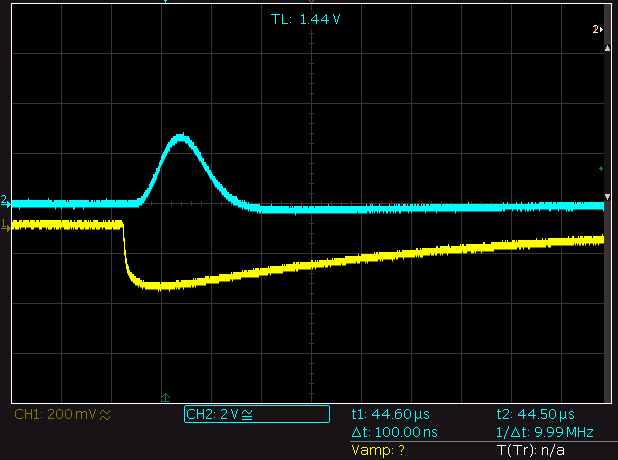
\includegraphics[width=0.6\textwidth]{../img/SCR0013.PNG}
  \caption[---]{Ausgangssignal des NaJ-Szintillators (gelb) und Signal am unipolaren Ausgang des Verstärkers (blau).}
  \label{img:najunip}
\end{center}
\end{figure}

\autoref{img:najbiptu} zeigt ebenfalls ein Signal des NaJ-Kristalls,
dann aber das verstärkte Signal am \emph{bipolaren} Ausgang des Verstärkers.
Man erkennt, dass das Maximum des bipolaren Signals schneller erreicht ist als das des unipolaren Signals;
der Abstand zum Einsatz des Szintillatorsignals beträgt hier nur 80\,ns (dies liegt daran,
dass das bipolare Signal die Ableitung des Unipolaren ist und bereits am Wendepunkt des Unipolaren sein Maximum
annimmt).\\
Das bipolare Signal wird mit dem Eingang des SCAs verbunden und dort zu einem Rechteckspuls geformt.
Da der Puls noch nicht schön geformt ist, bekommt er in der \emph{timing unit} eine schönere Form und eine Länge von
20\,ns. Dieser Puls ist auch auf \autoref{img:najbiptu} gezeigt.
\autoref{img:najbipsca2} zeigt die gleichen Signale in größerer Auflösung.
Hier lässt sich die zeitliche Verzögerung zwischen Einsetzen des Szintillatorsignals und Rechteckspuls
gut ablesen: Sie beträgt 130\,ns.

\begin{figure}[H]
\begin{center}
  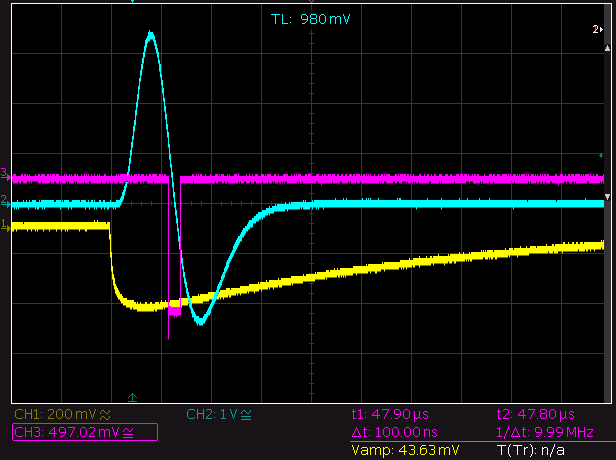
\includegraphics[width=0.6\textwidth]{../img/SCR0023.PNG}
  \caption[---]{Ausgangssignal des NaJ-Szintillators (gelb),
  Signal am bipolaren Ausgang des Verstärkers (blau)
  und Rechteckspuls nach der \emph{timing unit} (rosa).}
  \label{img:najbiptu}
\end{center}
\end{figure}

\begin{figure}[H]
\begin{center}
  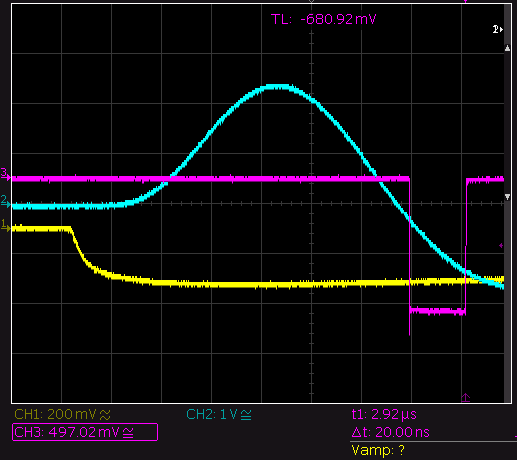
\includegraphics[width=0.6\textwidth]{../img/SCR0025.PNG}
  \caption[---]{Vergrößerter Ausschnitt aus \autoref{img:najbiptu} zur Bestimmung der Zeitverzögerung zwischen
  Einsatz des Szintillatorsignals (gelb) und Rechteckspuls (rosa) (135\,ns).}
  \label{img:najbipsca2}
\end{center}
\end{figure}

\begin{figure}[H]
\begin{center}
  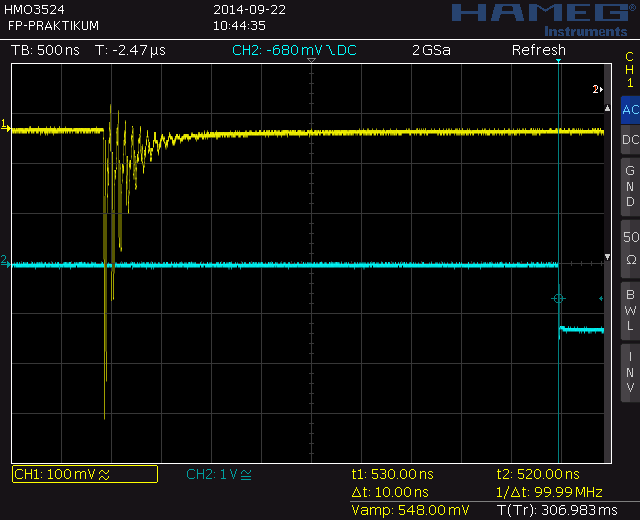
\includegraphics[width=0.6\textwidth]{../img/SCR0049.PNG}
  \caption[---]{Ausgangssignal des Plastik-Szintillators (gelb) und
  Rechteckspuls nach der \emph{timing unit} (blau) zur Bertimmung der Zeitverzögerung (90\,ns).}
  \label{img:plastiktu}
\end{center}
\end{figure}


Analog zum Anschluss der Geräte nach dem NaJ-Szintillator wird der gleiche Aufbau nach dem Plastikszintillator
aufgebaut. Das Signal des Plastikszintillators ist auf \autoref{img:plastiktu} zu sehen:
Im Vergleich zum NaJ-Szintillator ist die Amplitude hier viel höher (ca.~3\,V),
die Signallänge ist aber nur wenig mehr als 10\,ns.
Als Verstärkungsfaktor für diesen Szintillator wurde 10\,$\cdot$\,100 gewählt.\\
Auf \autoref{img:plastiktu} ist außerdem der Rechteckspuls nach der \emph{timing unit} zu sehen.
Er kommt hier schneller an als beim anderen Szintillator, 
die Laufzeit beträgt nur 90\,ns. Dieser Laufzeitunterschied wird dann am SCA mit der
Einstellung für das \emph{delay} auf 135\,ns verlängert, so dass zwei Signale, die von der selben
Elektron-Positron-Annihilation stammen, auch gleichzeitig an der Koinzidenzeinheit eintreffen.\\
Hier liegt eine weitere kritische Einstellmöglichkeit der Schaltung:
Die Koinzidenzeinheit liefert einen Puls an den Zähler, wenn an ihr zwei Rechteckspulse eintreffen,
die eine zeitliche Überschneidung besitzen.
Die Laufzeit der Signale, die für beide Szintillatoren auf 135\,ns eingestellt wurde,
schwankt allerdings um ca. 5\,ns. Wird die Breite der Rechteckspulse zu gering eingestellt, so
kann es sein, dass sie sich an der Koinzidenzeinheit nicht überschneiden und somit fälschlicherweise nicht
gezählt werden. Ist die Pulsbreite zu hoch, so werden sehr viele zufällige Koinzidenzen registriert.
Die Pulsbreite von 20\,ns erwies sich als optimal.\\
\autoref{img:koinzidenzen} zeigt Signale, die an der Koinzidenzeinheit ankommen:
Die Pulse, die in der Mitte der Abbildung liegen, sind koinzident.
Das Signal am rechten Rand ist zufällig, aber weit genug entfernt, um nicht registriert zu werden.

\begin{figure}[H]
\begin{center}
  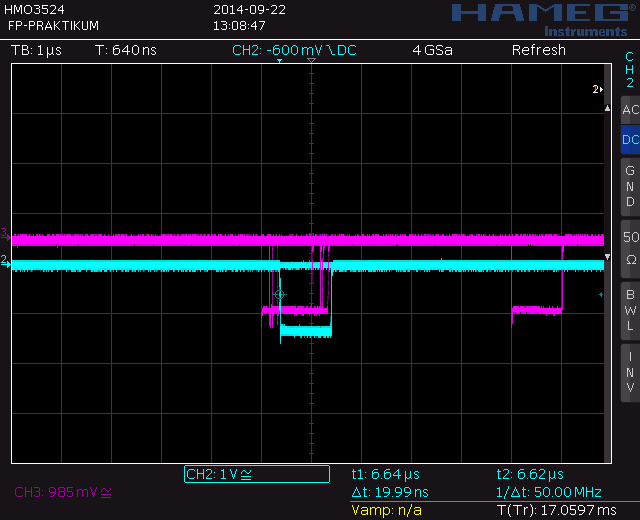
\includegraphics[width=0.6\textwidth]{../img/SCR0059.PNG}
  \caption[---]{Eingangssignale an der Koinzidenzeinheit: Sich überschneidende Rechteckspulse werden als
  Koinzidenzen registriert. Der Puls am rechten Rand ist zufällig und wird nicht registriert.}
  \label{img:koinzidenzen}
\end{center}
\end{figure}